% Source: tex/chapters/ch06/08_実務上の考慮.tex
\subsubsection{ソフトウェアエンジニアリング運用の自動化}

現代の運用では、自動化が中心的役割を持つ。環境構築、ユーザアカウント作成、サーバ準備、実行時設定変更、配備、試験、デバッグ支援などを自動化できる。ソフトウェア技術者は、アプリケーション自動化と運用自動化を結びつけることで大きな効果を得る。

運用自動化の傾向は、複雑さを減らし、インフラ準備を速め、開発者へ運用サービススクリプトを提供し、アプリケーション定義、配備、試験作業を自動化する方向にある。

\begin{figure}[htbp]
\centering
\IfFileExists{assets/fig-ch06-11.png}{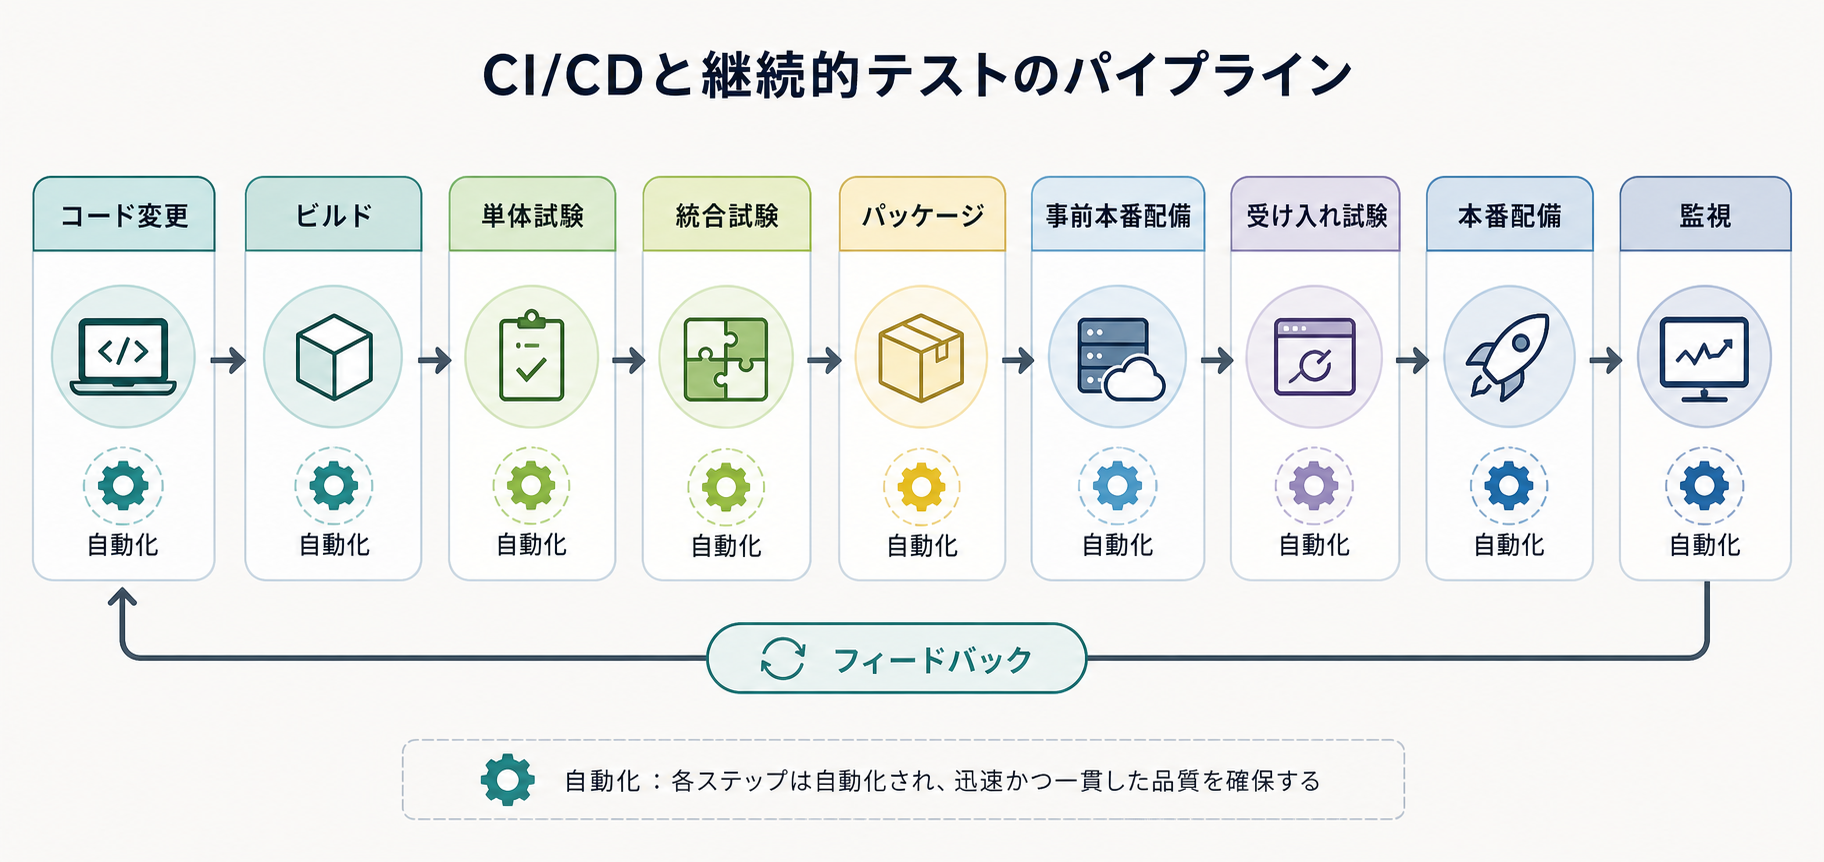
\includegraphics[width=0.96\linewidth]{assets/fig-ch06-11.png}}{\fbox{\parbox[c][48mm][c]{0.9\linewidth}{\centering 画像生成待ち\\CI/CDと継続的テストのパイプライン}}}
\caption{CI/CDと継続的テストのパイプライン}
\label{fig:ch06-11}
\end{figure}
